\chapter{Conclusions and Future Work}
\label{chapter:conclusion}

\section{Thesis Revisited}
Modern software systems come with a lot of configuration options, which can be tweaked to modify the functional or
non-functional (e.g., throughput or runtime) requirements. Finding
the good or optimal configuration to run a particular workload is essential
since there is a significant difference between the best and the
worst configurations. Many researchers report that modern software
systems come with a daunting number of configuration options~\cite{xu2015hey}.
The size of the configuration space increases exponentially with the
number of configuration options. The long runtimes or cost required
to run benchmarks make this problem more challenging.

Prior work in this area used a machine learning method
to model the configuration space accurately. The model is built sequentially,
where new configurations are sampled randomly, and the
quality or accuracy of the model is measured using a holdout set. This strategy
makes these methods unsuitable in a practical setting since they can be very expensive. On the other hand, there are software systems for which an accurate model cannot be
built.

In this thesis, we introduced techniques and method, which can find good configurations while minimizing the search cost. The central insight of this thesis is: to build a machine learning model (not accurate) which
can differentiate between the good and not so good solutions. 

The important lessons, we learned during the preparation of the thesis are:
\begin{itemize}
    \item \textbf{Clustering: } Early attempts managed to use random sampling along with machine learning models to build accurate models, which can then be used to find good configurations. However, random sampling and accurate machine learning models can lead to an expensive model building process. We attempt to \textbf{reduce the cost of the model building by adding the idea of stratified sampling instead of random sampling} i.e.; we try to cluster the configuration space using a top-down clustering and sampling from each sub-population. We have found stratified sampling can significantly reduce the cost of model building and also reduce the variance in the model built. \\
    \noindent\textbf{Lessons Learned: } Even though we found the stratified sampling approach of \what works for the software systems explored in our paper~\cite{nair2017faster}. However, while performing external validation (with a more diverse set of software systems), we found that \what is not efficient (as shown by our preliminary study). Upon further investigation, we found that we make an important assumption: ``our clustering algorithm (WHERE in our case) returns meaningful cluster''. This assumption meant that we know the distance function applicable to the configuration space, i.e., configurations with shorter distance is similar to the configurations with a larger distance. The ineffectiveness of \what is primarily because our assumption did not hold for the newer configuration spaces.
    
    \item \textbf{Ranking: } A retrospective look on the prior work including our work, made us realize that researchers have been tackling the problem of finding good configuration by transforming the problem to a building accurate model problem. However, the fundamental idea in this work is to use ranking as an approach for building models. The ranking is a useful paradigm to solve the software configuration optimization because (1) ranking is the ultimate goal, (2) Ranking is extremely robust since it is only mildly affected by errors or outliers, and (3) Ranking reduces the number of training samples required to train a model.\\
    \noindent\textbf{Lessons Learned:} The model is built sequentially, where new configurations are sampled randomly, and the quality or accuracy of the model is measured using a holdout set. The size of the holdout set in some cases could be up to 20\% of the configuration space and need to be evaluated (i.e., measured) before even the machine learning model is entirely built. This strategy makes these methods unsuitable in a practical setting since the generated holdout set can be (very) expensive. 
    
    \item \textbf{Sequential Model-based Optimization:}  The problem of finding the (near) optimal configuration is expensive and often infeasible using the current techniques. A useful strategy could be to build a machine learning model which can differentiate between the good and not so good solutions. \flash, a Sequential Model-based Optimization (SMBO), is a useful strategy to find extremes of an unknown objective. \flash is efficient because of its ability to incorporate prior belief as already measured solutions (or configurations), to help direct further sampling. Here, the prior represents the already known areas of the search (or performance optimization) problem. The prior can be used to estimate the rest of the points (or unevaluated configurations). Once one (or many) points are evaluated based on the prior, the posterior can be defined. The posterior captures the updated belief in the objective function. This step is performed by using a machine learning model, also called \textit{surrogate model}. The concept of \flash can be simply stated as:
    \begin{itemize}
        \item Given what one knows about the problem,
        \item what can be done next?
    \end{itemize}
    The ``given what one knows about the problem'' part is achieved by using a machine learning model whereas ``what can be done next'' is performed by an acquisition function. Such acquisition function automatically adjusts the exploration (``should we sample in uncertain parts of the search space'') and exploitation (``should we stick to what is already known'') behavior of the method.\\
    \noindent\textbf{Lessons Learned: } Much current research (including all the approaches discussed in this thesis) has explored this problem, usually by creating performance models that predict performance characteristics. While this approach is cheaper and more effective than manual configuration, it still incurs the expensive of extensive data collection about the software. This is undesirable since this data collection has to be repeated if ever the software is updated on the workload of the system changes abruptly. In such a scenario, all prior research suffers from the same drawback: these approaches do not learn from previous optimization experiments and must be rerun whenever the environment of the experiments change. Note our use of the term environment. This refers to the external factors influencing the performance of the system such as workload, hardware, version of the software.
    
\end{itemize}


\section{Future Work}
There are many fruitful avenues of research that are worthwhile to pursue but
beyond the scope of this dissertation. Here are just a few directions: 

\noindent\textbf{Can expert knowledge be used to increase the rate of convergence?}\\
During our many conversations with the people in the industry, we get pushback regarding the automated approaches. The common theme of this conversation is generally, ``we have been configuring our software systems for decades, and we have people who can configure these systems in their sleep''. While this line of reasoning is generally flawed and there are several pieces of evidence (as discussed in our related work session). Pooyan Jamshidi has shown several such examples. Figure~\ref{fig:expert_wrong} is one such example with Cassandra.
\begin{figure}[t]
\centering
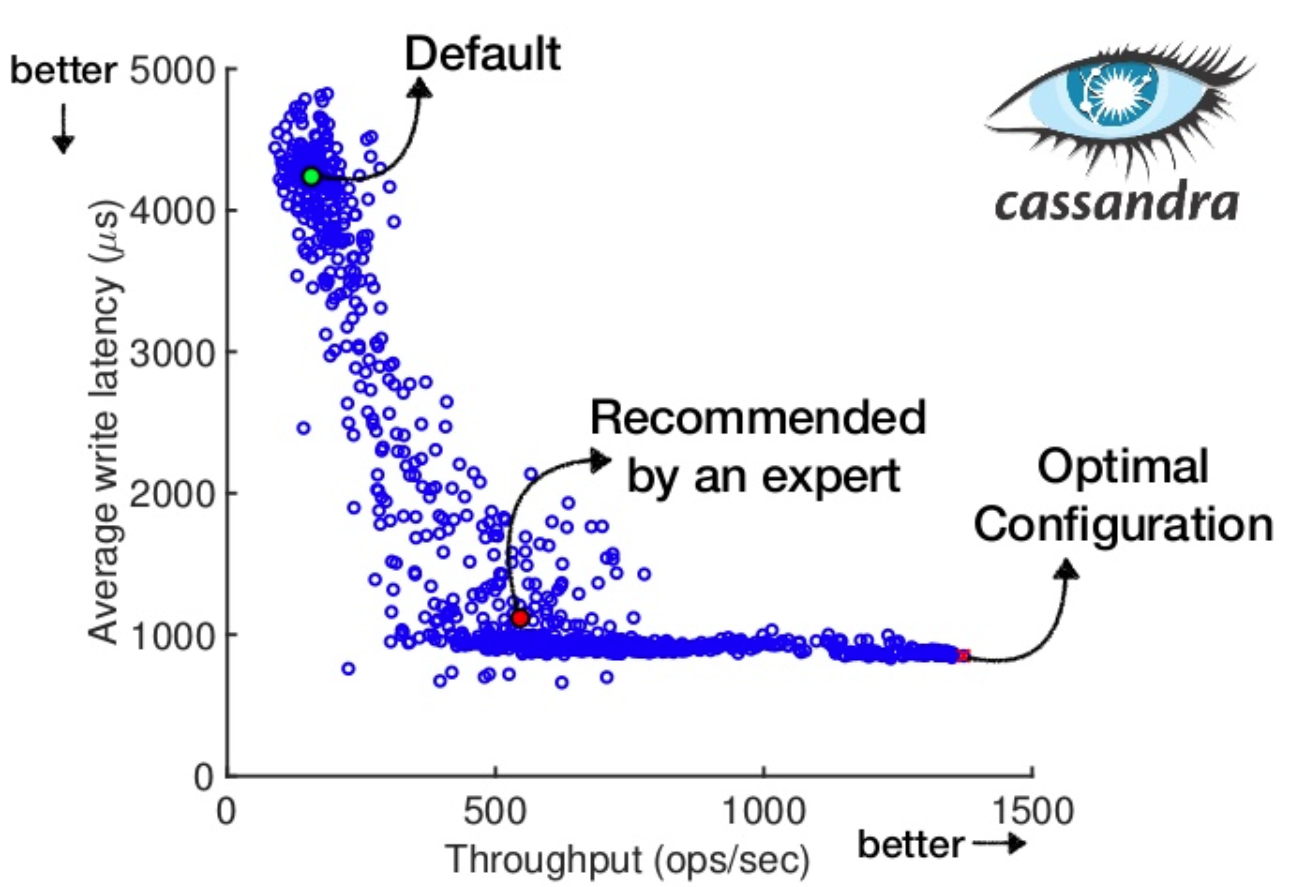
\includegraphics[width=\columnwidth]{Chapter-Conclusion/Figures/ExpertWrong.png}
\caption[Comparison between default configurations,  configurations selected by experts and optimal configuration.]{Comparison between default configurations,  configurations selected by experts and optimal configuration. From \url{http://tiny.cc/existingTechniques}.
}
\label{fig:expert_wrong}
\end{figure}
However, the rate of convergence is \flash is dependent on the initial configurations (currently selected using random sampling). So, if expert knowledge can be successfully extracted and embedded into the initial sample, it can further reduce the cost of optimization. There has been some effort made in this direction~\cite{feurer2018scalable, Hsu2018Scout}.

\noindent\textbf{Can we learn from our experience to increase the rate of convergence or decrease the cost?}\\
Transfer learning can only be useful in cases where the source environment is similar to the target environment. If the source and the target are not similar, knowledge should not be transferred. In such an extreme situation, transfer learning can be unsuccessful and can lead to a \textit{negative transfer}. Prior work on transfer learning focused on ``What to transfer'' and ``How to transfer'', by implicitly assuming that the source and target are related to each other. Hence, that work failed to address “When to transfer.” Jamshidi et al.~\cite{jamshidi2017transfer} alluded to this and explained when transfer learning
works but, did not provide a method which can help in selecting a
suitable source. There is a need for some effort in solving the problem of performance optimization by choosing an appropriate source to transfer knowledge. We have made some progress in this area~\cite{nair2018transfer}.

\noindent\textbf{Does learning about landscape~\footnote{Landscape refers to features of the problem such as modality (local optimal and plateau), basins of attractions~\cite{mersmann2011exploratory}} provide us with information about which search strategy to use?}\\
The techniques used in \flash (model and the acquisition function) is a subset of a larger space of options. During the development phase of \flash, we tried various options and narrowed down on the existing options using trial and error. However, there may be configuration spaces where \flash is not effective. Since the configuration space is currently a black box to us, there is a need for a fast technique to sample and understand that \textbf{landspace} quickly. This information can then be used to select the right combination of model and acquisition function. This problem is currently explored as a different problem namely algorithm configuration, and there is some progress in this area~\cite{mersmann2011exploratory}. There is also a great tool available to get a head start in this domain~\cite{hanster2017flaccogui}.

\noindent\textbf{Can these ideas be applied to other domains?}\\
In an abstract sense, the problems discussed in this thesis falls under a broad realm of black-box optimization. The only challenging component (or rather a constraint) to this problem is each evaluation is costly. Hence, we need to be aware of the cost (both time and computing resources). There are various other domains where the methods, discussed in this thesis, can be applied such as hyperparameter tuning, cloud configuration, etc. We made some progress in applying these techniques in the cloud configuration~\cite{Hsu2018Arrow, Hsu2018Micky, Hsu2018Scout}. 

\noindent\textbf{How to optimize for a large macro-system which involves many micro-systems?}
The software systems, explored in this thesis, are standalone system and not a collection of heterogeneous systems. We hypothesize that in such collective systems the configuration of one of the participating software system can affect the performance of another participating software system. In such cases, how can we alter the techniques discussed in this thesis to be valuable in such situations. 

\section{Epilogue}
The prior works in the area of performance optimization have transformed the problem of finding good configurations into a modeling problem. Researchers have tried to solve this problem by building accurate models, which made this process of optimization (using models) expensive. In this thesis, we have shown that the problem of performance optimization can be tacked as an optimization problem and not a modeling problem. This can be done by building inaccurate models and use the models to explore new regions of the configuration space. 

The idea of this thesis can be best encapsulated as: 
\begin{center}
\begin{flushleft}
    \hspace{1.5cm}\textbf{``There's no sense in being precise when you }\\
    \hspace{1.5cm}\textbf{don't even know what you're talking about.''}\\
    \hspace{1.5cm}\hfill\textbf{--- John von Neumann}\\
\end{flushleft}
\end{center}

% 5. It is always difficult to know which configurations are truly valid? So, given specific examples of valid configuration can build a model which could potentially tell us which configurations could be valid or not? Some form of a classification model?
% 7. Given that the performance of a particular system running a specific benchmark is highly variable (because of its environment, for example, variability in cloud xxxbubbleup) how can we build models which can tolerate multiple levels of fidelity?